\section{sim.h File Reference}
\label{sim_8h}\index{sim.h@{sim.h}}
{\tt \#include $<$stdint.h$>$}\par
{\tt \#include $<$stdio.h$>$}\par
{\tt \#include $<$setjmp.h$>$}\par
{\tt \#include $<$time.h$>$}\par
{\tt \#include \char`\"{}options.h\char`\"{}}\par
{\tt \#include \char`\"{}stats.h\char`\"{}}\par
{\tt \#include \char`\"{}regs.h\char`\"{}}\par
{\tt \#include \char`\"{}memory.h\char`\"{}}\par
{\tt \#include \char`\"{}thread.h\char`\"{}}\par
{\tt \#include \char`\"{}../kernel/clock.h\char`\"{}}\par


Include dependency graph for sim.h:\nopagebreak
\begin{figure}[H]
\begin{center}
\leavevmode
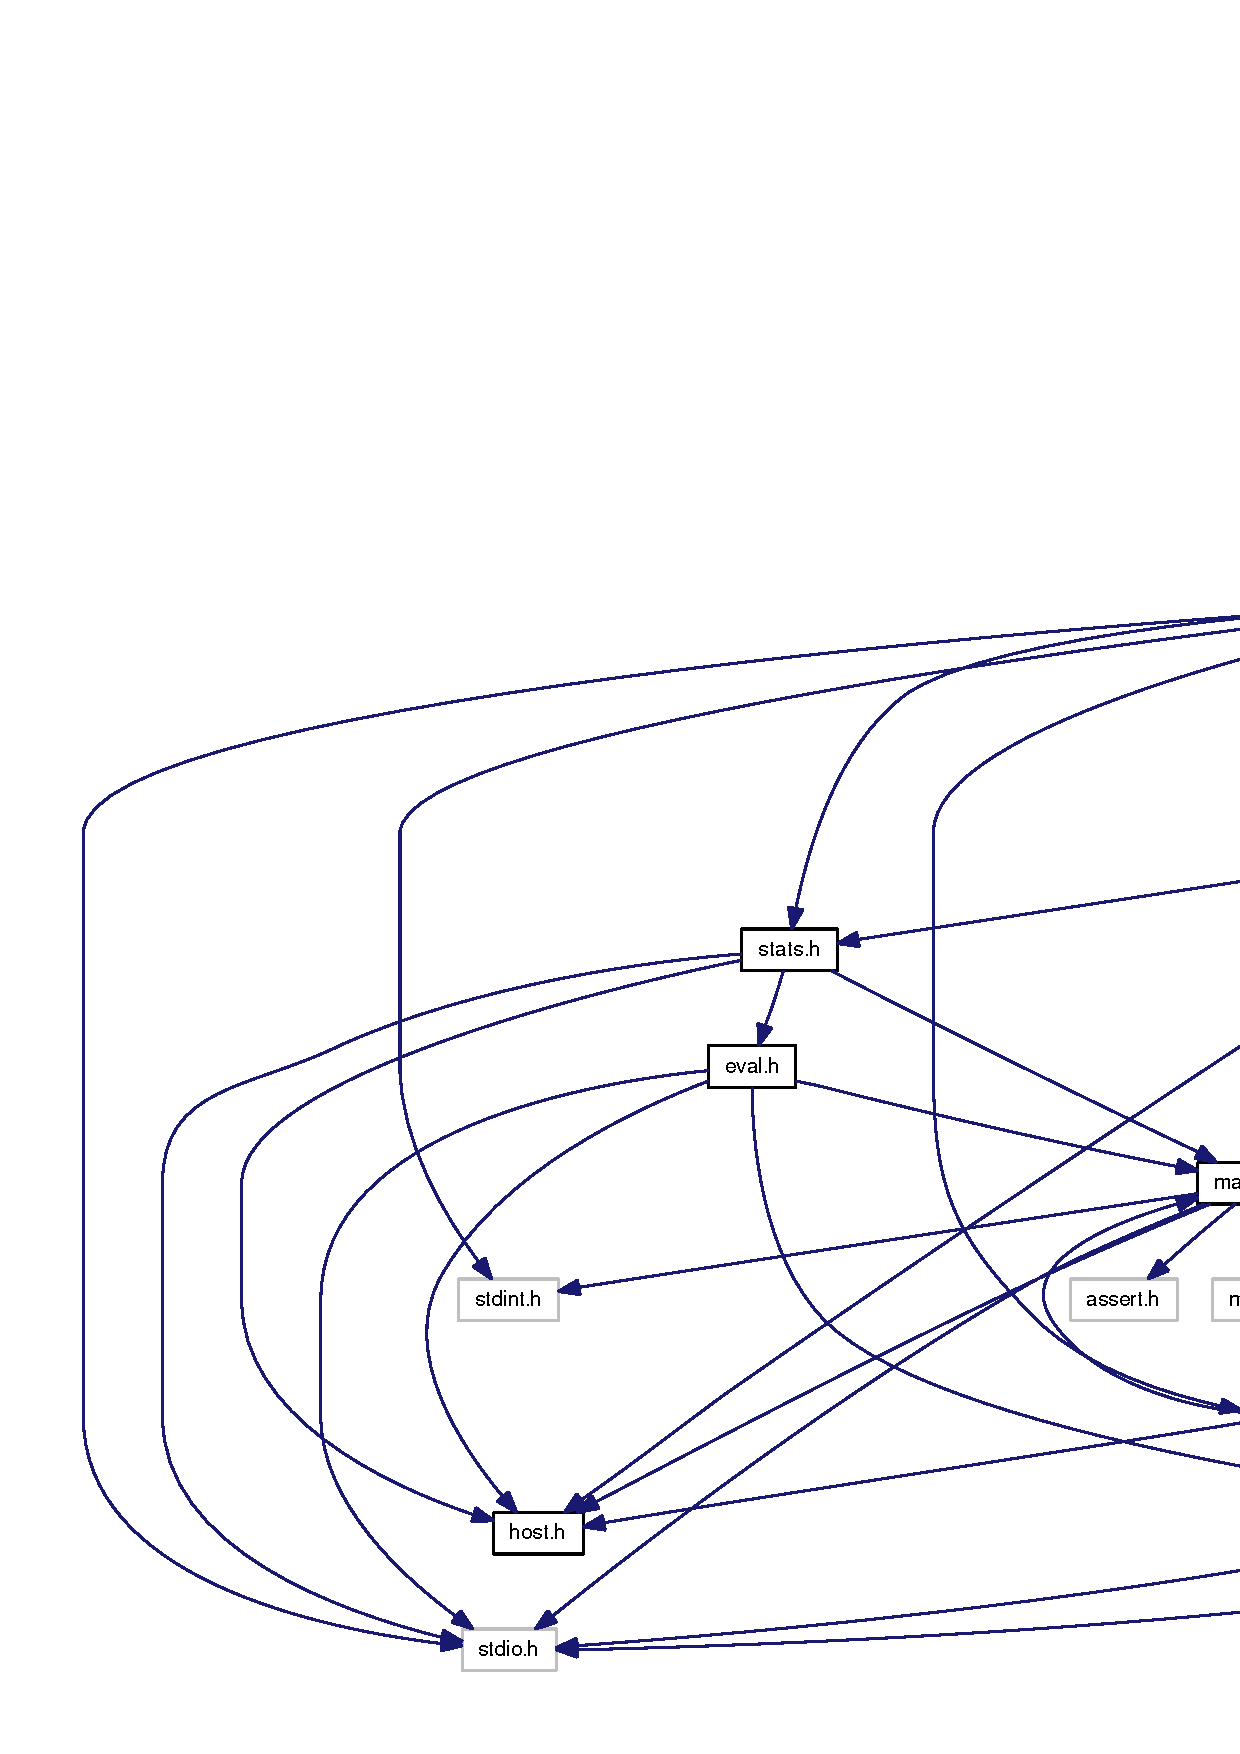
\includegraphics[width=420pt]{sim_8h__incl}
\end{center}
\end{figure}


This graph shows which files directly or indirectly include this file:\nopagebreak
\begin{figure}[H]
\begin{center}
\leavevmode
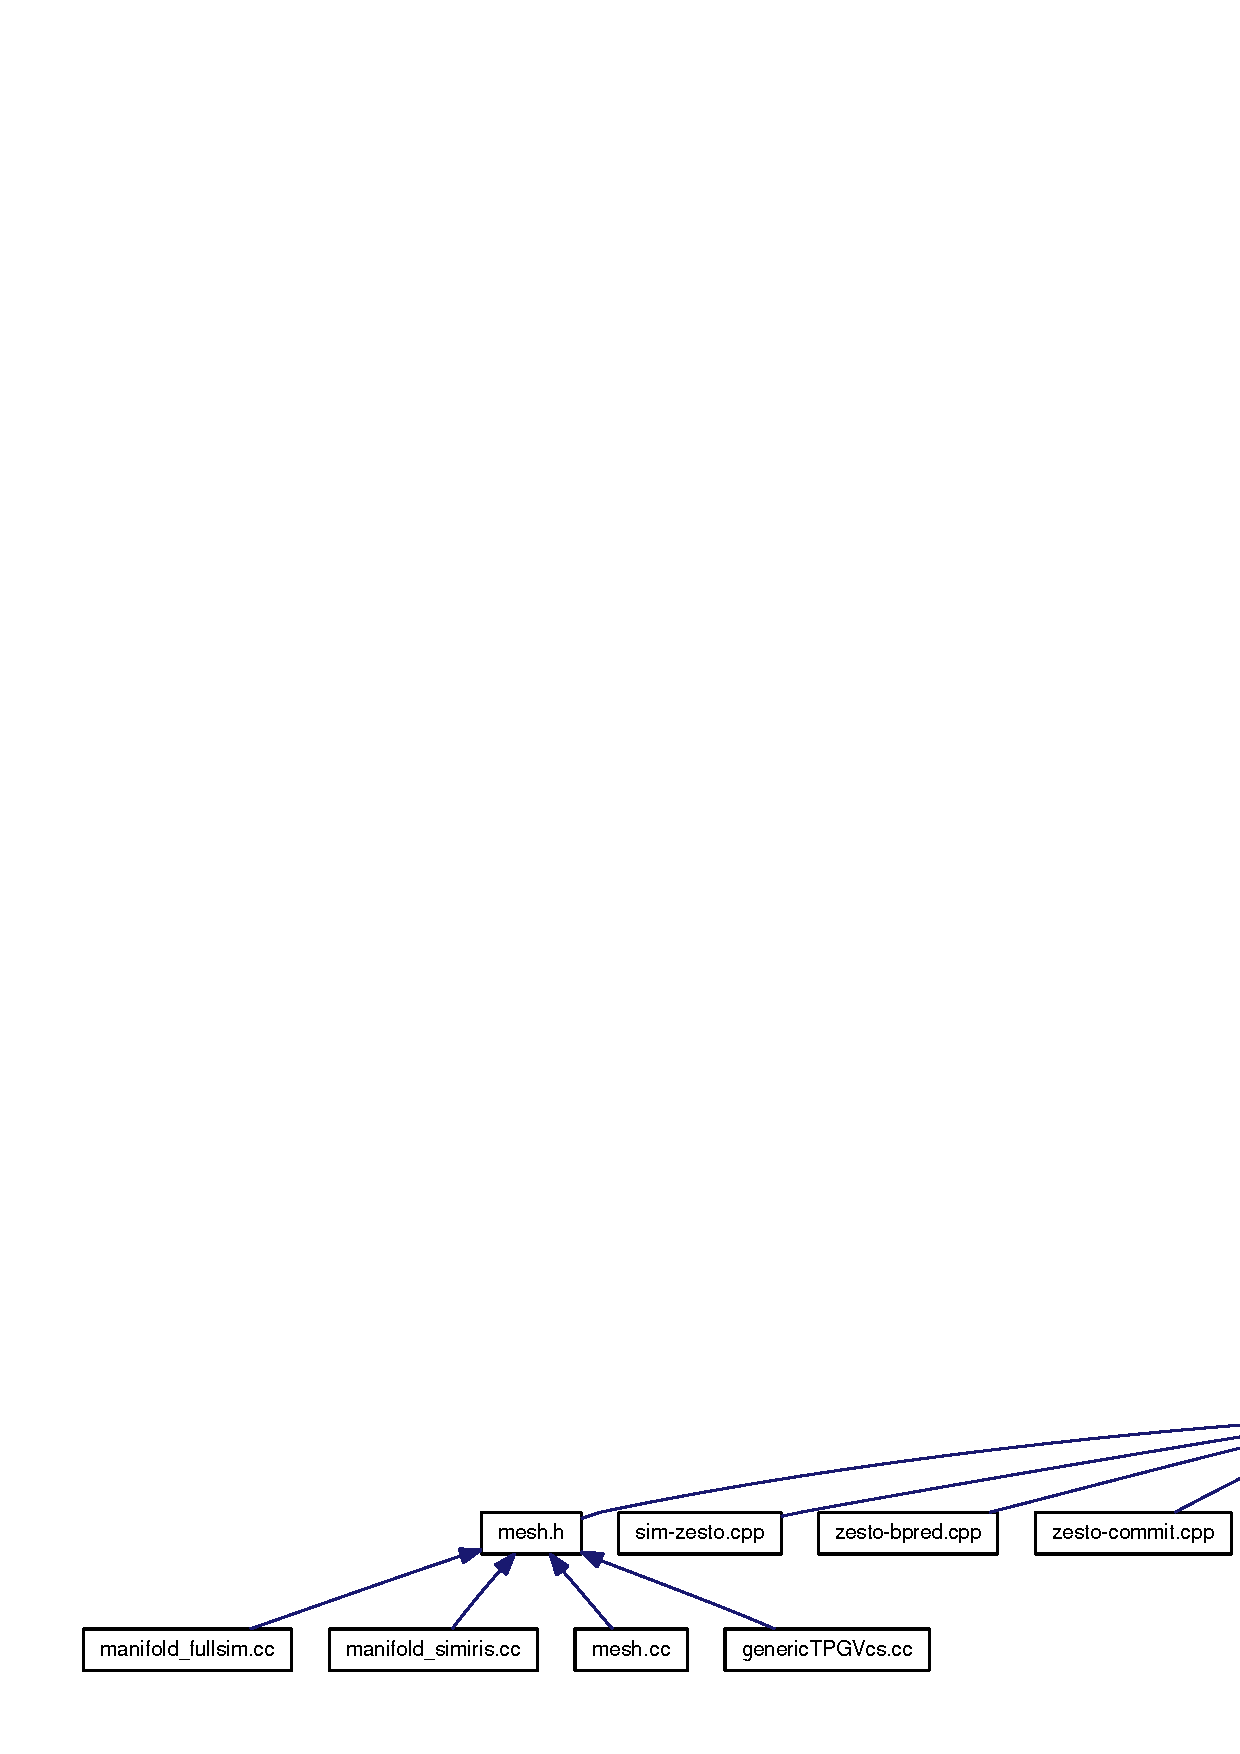
\includegraphics[width=420pt]{sim_8h__dep__incl}
\end{center}
\end{figure}
\subsection*{Classes}
\begin{CompactItemize}
\item 
class {\bf zesto\_\-component}
\end{CompactItemize}
\subsection*{Defines}
\begin{CompactItemize}
\item 
\#define {\bf NICE\_\-DEFAULT\_\-VALUE}~0
\end{CompactItemize}
\subsection*{Functions}
\begin{CompactItemize}
\item 
void {\bf sim\_\-reg\_\-options} (struct {\bf opt\_\-odb\_\-t} $\ast$odb)
\item 
void {\bf sim\_\-check\_\-options} (struct {\bf opt\_\-odb\_\-t} $\ast$odb, int argc, char $\ast$$\ast$argv)
\item 
void {\bf sim\_\-reg\_\-stats} (struct {\bf thread\_\-t} $\ast$$\ast${\bf cores}, struct {\bf stat\_\-sdb\_\-t} $\ast$sdb)
\item 
void {\bf sim\_\-pre\_\-init} (void)
\item 
void {\bf sim\_\-post\_\-init} (void)
\item 
void {\bf sim\_\-aux\_\-config} (FILE $\ast$stream)
\item 
void {\bf sim\_\-main} (void)
\item 
void {\bf sim\_\-aux\_\-stats} (FILE $\ast$stream)
\item 
void {\bf sim\_\-uninit} (void)
\item 
void {\bf sim\_\-print\_\-stats} (FILE $\ast$fd)
\end{CompactItemize}
\subsection*{Variables}
\begin{CompactItemize}
\item 
double {\bf cpu\_\-speed}
\item 
int {\bf sim\_\-dump\_\-stats}
\item 
int {\bf sim\_\-exit\_\-now}
\item 
jmp\_\-buf {\bf sim\_\-exit\_\-buf}
\item 
int {\bf sim\_\-swap\_\-bytes}
\item 
int {\bf sim\_\-swap\_\-words}
\item 
time\_\-t {\bf sim\_\-start\_\-time}
\item 
time\_\-t {\bf sim\_\-end\_\-time}
\item 
int {\bf sim\_\-elapsed\_\-time}
\item 
struct {\bf opt\_\-odb\_\-t} $\ast$ {\bf sim\_\-odb}
\item 
struct {\bf stat\_\-sdb\_\-t} $\ast$ {\bf sim\_\-sdb}
\item 
char $\ast$ {\bf sim\_\-eio\_\-fname} [MAX\_\-CORES]
\item 
FILE $\ast$ {\bf sim\_\-eio\_\-fd} [MAX\_\-CORES]
\item 
FILE $\ast$ {\bf sim\_\-progfd}
\item 
bool {\bf help\_\-me}
\item 
int {\bf rand\_\-seed}
\item 
bool {\bf init\_\-quit}
\item 
int {\bf nice\_\-priority}
\item 
char $\ast$ {\bf sim\_\-simout}
\item 
char $\ast$ {\bf sim\_\-progout}
\item 
unsigned int {\bf vcs}
\item 
unsigned int {\bf ports}
\item 
unsigned int {\bf buffer\_\-size}
\item 
unsigned int {\bf credits}
\item 
unsigned int {\bf no\_\-nodes}
\item 
unsigned int {\bf no\_\-mcs}
\item 
unsigned long long int {\bf max\_\-sim\_\-time}
\item 
unsigned int {\bf MC\_\-ADDR\_\-BITS}
\item 
unsigned int {\bf BANK\_\-BITS}
\item 
unsigned int {\bf THREAD\_\-BITS\_\-POSITION}
\item 
unsigned int {\bf do\_\-two\_\-stage\_\-router}
\item 
unsigned int {\bf max\_\-phy\_\-link\_\-bits}
\item 
unsigned int {\bf print\_\-setup}
\item 
unsigned int {\bf grid\_\-size}
\item 
unsigned int {\bf cores\_\-per\_\-node}
\end{CompactItemize}


\subsection{Define Documentation}
\index{sim.h@{sim.h}!NICE\_\-DEFAULT\_\-VALUE@{NICE\_\-DEFAULT\_\-VALUE}}
\index{NICE\_\-DEFAULT\_\-VALUE@{NICE\_\-DEFAULT\_\-VALUE}!sim.h@{sim.h}}
\subsubsection[{NICE\_\-DEFAULT\_\-VALUE}]{\setlength{\rightskip}{0pt plus 5cm}\#define NICE\_\-DEFAULT\_\-VALUE~0}\label{sim_8h_d532132f299e8f6d3961f66ef637f5aa}




Definition at line 115 of file sim.h.

\subsection{Function Documentation}
\index{sim.h@{sim.h}!sim\_\-aux\_\-config@{sim\_\-aux\_\-config}}
\index{sim\_\-aux\_\-config@{sim\_\-aux\_\-config}!sim.h@{sim.h}}
\subsubsection[{sim\_\-aux\_\-config}]{\setlength{\rightskip}{0pt plus 5cm}void sim\_\-aux\_\-config (FILE $\ast$ {\em stream})}\label{sim_8h_67e5d7a21600d2eb1fb2f0798fc24a7c}




Definition at line 423 of file sim-zesto.cpp.\index{sim.h@{sim.h}!sim\_\-aux\_\-stats@{sim\_\-aux\_\-stats}}
\index{sim\_\-aux\_\-stats@{sim\_\-aux\_\-stats}!sim.h@{sim.h}}
\subsubsection[{sim\_\-aux\_\-stats}]{\setlength{\rightskip}{0pt plus 5cm}void sim\_\-aux\_\-stats (FILE $\ast$ {\em stream})}\label{sim_8h_f0d3b44eaaad1fd53b38c9f82deb05fd}




Definition at line 430 of file sim-zesto.cpp.\index{sim.h@{sim.h}!sim\_\-check\_\-options@{sim\_\-check\_\-options}}
\index{sim\_\-check\_\-options@{sim\_\-check\_\-options}!sim.h@{sim.h}}
\subsubsection[{sim\_\-check\_\-options}]{\setlength{\rightskip}{0pt plus 5cm}void sim\_\-check\_\-options (struct {\bf opt\_\-odb\_\-t} $\ast$ {\em odb}, \/  int {\em argc}, \/  char $\ast$$\ast$ {\em argv})}\label{sim_8h_d6c7eccd0fa4b587be632b532e3b3e04}




Referenced by main().

Here is the caller graph for this function:\nopagebreak
\begin{figure}[H]
\begin{center}
\leavevmode
\includegraphics[width=109pt]{sim_8h_d6c7eccd0fa4b587be632b532e3b3e04_icgraph}
\end{center}
\end{figure}
\index{sim.h@{sim.h}!sim\_\-main@{sim\_\-main}}
\index{sim\_\-main@{sim\_\-main}!sim.h@{sim.h}}
\subsubsection[{sim\_\-main}]{\setlength{\rightskip}{0pt plus 5cm}void sim\_\-main (void)}\label{sim_8h_6b9951fa76e6d8b400f13df1c975ed3b}




Definition at line 1006 of file sim-zesto.cpp.

References core\_\-t::current\_\-thread, fastfwd, fatal(), core\_\-t::fetch, MD\_\-FETCH\_\-NEXT\_\-PC, num\_\-threads, core\_\-fetch\_\-t::PC, thread\_\-t::pin\_\-trace, thread\_\-t::regs, regs\_\-t::regs\_\-NPC, regs\_\-t::regs\_\-PC, sim\_\-fastfwd(), sim\_\-start\_\-time, store\_\-nextPC, and use\_\-stored\_\-nextPC.

Referenced by main().

Here is the caller graph for this function:\nopagebreak
\begin{figure}[H]
\begin{center}
\leavevmode
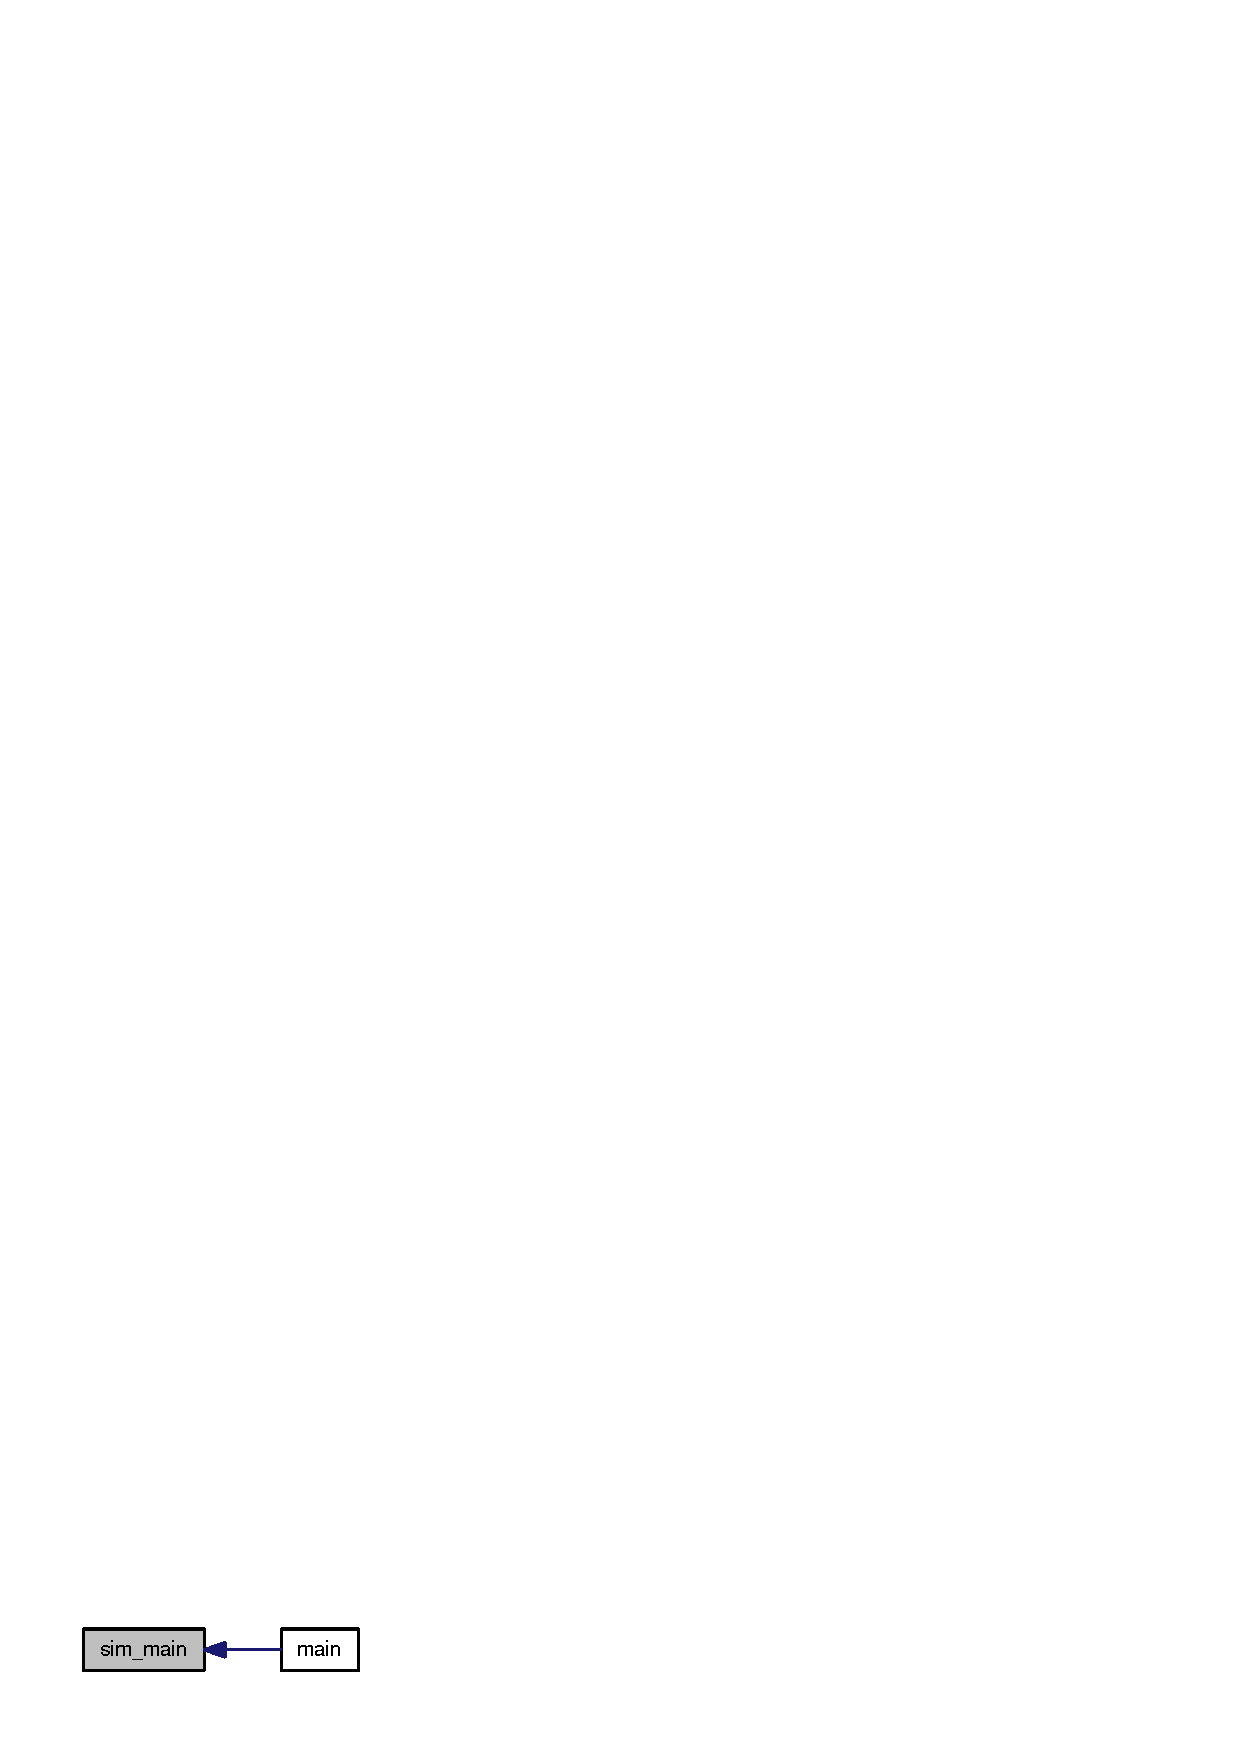
\includegraphics[width=88pt]{sim_8h_6b9951fa76e6d8b400f13df1c975ed3b_icgraph}
\end{center}
\end{figure}
\index{sim.h@{sim.h}!sim\_\-post\_\-init@{sim\_\-post\_\-init}}
\index{sim\_\-post\_\-init@{sim\_\-post\_\-init}!sim.h@{sim.h}}
\subsubsection[{sim\_\-post\_\-init}]{\setlength{\rightskip}{0pt plus 5cm}void sim\_\-post\_\-init (void)}\label{sim_8h_7af633ff74aee8f90ea9a610892191ce}




Definition at line 330 of file sim-zesto.cpp.

References thread\_\-t::active, core\_\-t::alloc, alloc\_\-create(), BOOT\_\-PC, core\_\-t::commit, commit\_\-create(), uncore\_\-t::core, core\_\-t::core\_\-t(), cores\_\-per\_\-node, cpu\_\-speed, thread\_\-t::current\_\-core, core\_\-t::current\_\-thread, core\_\-t::decode, decode\_\-create(), core\_\-t::exec, exec\_\-create(), fatal(), core\_\-t::fetch, fetch\_\-create(), thread\_\-t::id, knobs, core\_\-t::knobs, core\_\-knobs\_\-t::model, my\_\-SIGSEGV\_\-handler(), no\_\-mcs, no\_\-nodes, num\_\-threads, core\_\-t::oracle, thread\_\-t::regs, regs\_\-init(), regs\_\-t::regs\_\-PC, core\_\-t::uncore, uncore\_\-t::uncore\_\-t(), and vcs.

Referenced by main().

Here is the caller graph for this function:\nopagebreak
\begin{figure}[H]
\begin{center}
\leavevmode
\includegraphics[width=96pt]{sim_8h_7af633ff74aee8f90ea9a610892191ce_icgraph}
\end{center}
\end{figure}
\index{sim.h@{sim.h}!sim\_\-pre\_\-init@{sim\_\-pre\_\-init}}
\index{sim\_\-pre\_\-init@{sim\_\-pre\_\-init}!sim.h@{sim.h}}
\subsubsection[{sim\_\-pre\_\-init}]{\setlength{\rightskip}{0pt plus 5cm}void sim\_\-pre\_\-init (void)}\label{sim_8h_6f8bfcc0d1d039d6fb378af082656f6f}




Definition at line 193 of file sim-zesto.cpp.

References core\_\-knobs\_\-t::alloc, core\_\-knobs\_\-t::bpred\_\-opt\_\-str, core\_\-knobs\_\-t::branch\_\-decode\_\-limit, core\_\-knobs\_\-t::byteQ\_\-linesize, core\_\-knobs\_\-t::byteQ\_\-size, core\_\-knobs\_\-t::commit, core\_\-knobs\_\-t::decode, core\_\-knobs\_\-t::decoders, core\_\-knobs\_\-t::depth, core\_\-knobs\_\-t::DL1\_\-MSHR\_\-cmd, core\_\-knobs\_\-t::DL1\_\-num\_\-PF, core\_\-knobs\_\-t::DL1PF\_\-opt\_\-str, core\_\-knobs\_\-t::DL2\_\-MSHR\_\-cmd, core\_\-knobs\_\-t::DL2\_\-num\_\-PF, core\_\-knobs\_\-t::DL2PF\_\-opt\_\-str, core\_\-knobs\_\-t::exec, core\_\-knobs\_\-t::fetch, core\_\-knobs\_\-t::fp\_\-penalty, core\_\-knobs\_\-t::fu\_\-bindings, FU\_\-FADD, FU\_\-FCPLX, FU\_\-FDIV, FU\_\-FMUL, FU\_\-IDIV, FU\_\-IEU, FU\_\-IMUL, FU\_\-JEU, FU\_\-LD, FU\_\-SHIFT, FU\_\-STA, FU\_\-STD, core\_\-knobs\_\-t::IL1\_\-num\_\-PF, core\_\-knobs\_\-t::IL1PF\_\-opt\_\-str, core\_\-knobs\_\-t::IQ\_\-size, core\_\-knobs\_\-t::issue\_\-rate, knobs, core\_\-knobs\_\-t::latency, core\_\-knobs\_\-t::LDQ\_\-size, MAX\_\-DECODE\_\-WIDTH, core\_\-knobs\_\-t::memory, memzero(), core\_\-knobs\_\-t::model, core\_\-knobs\_\-t::MS\_\-latency, core\_\-knobs\_\-t::num\_\-bpred\_\-components, core\_\-knobs\_\-t::num\_\-decoder\_\-specs, core\_\-knobs\_\-t::num\_\-exec\_\-ports, core\_\-knobs\_\-t::payload\_\-depth, core\_\-knobs\_\-t::port\_\-binding, core\_\-knobs\_\-t::ROB\_\-size, core\_\-knobs\_\-t::RS\_\-size, core\_\-knobs\_\-t::STQ\_\-size, core\_\-knobs\_\-t::target\_\-stage, core\_\-knobs\_\-t::uopQ\_\-size, and core\_\-knobs\_\-t::width.

Referenced by main().

Here is the caller graph for this function:\nopagebreak
\begin{figure}[H]
\begin{center}
\leavevmode
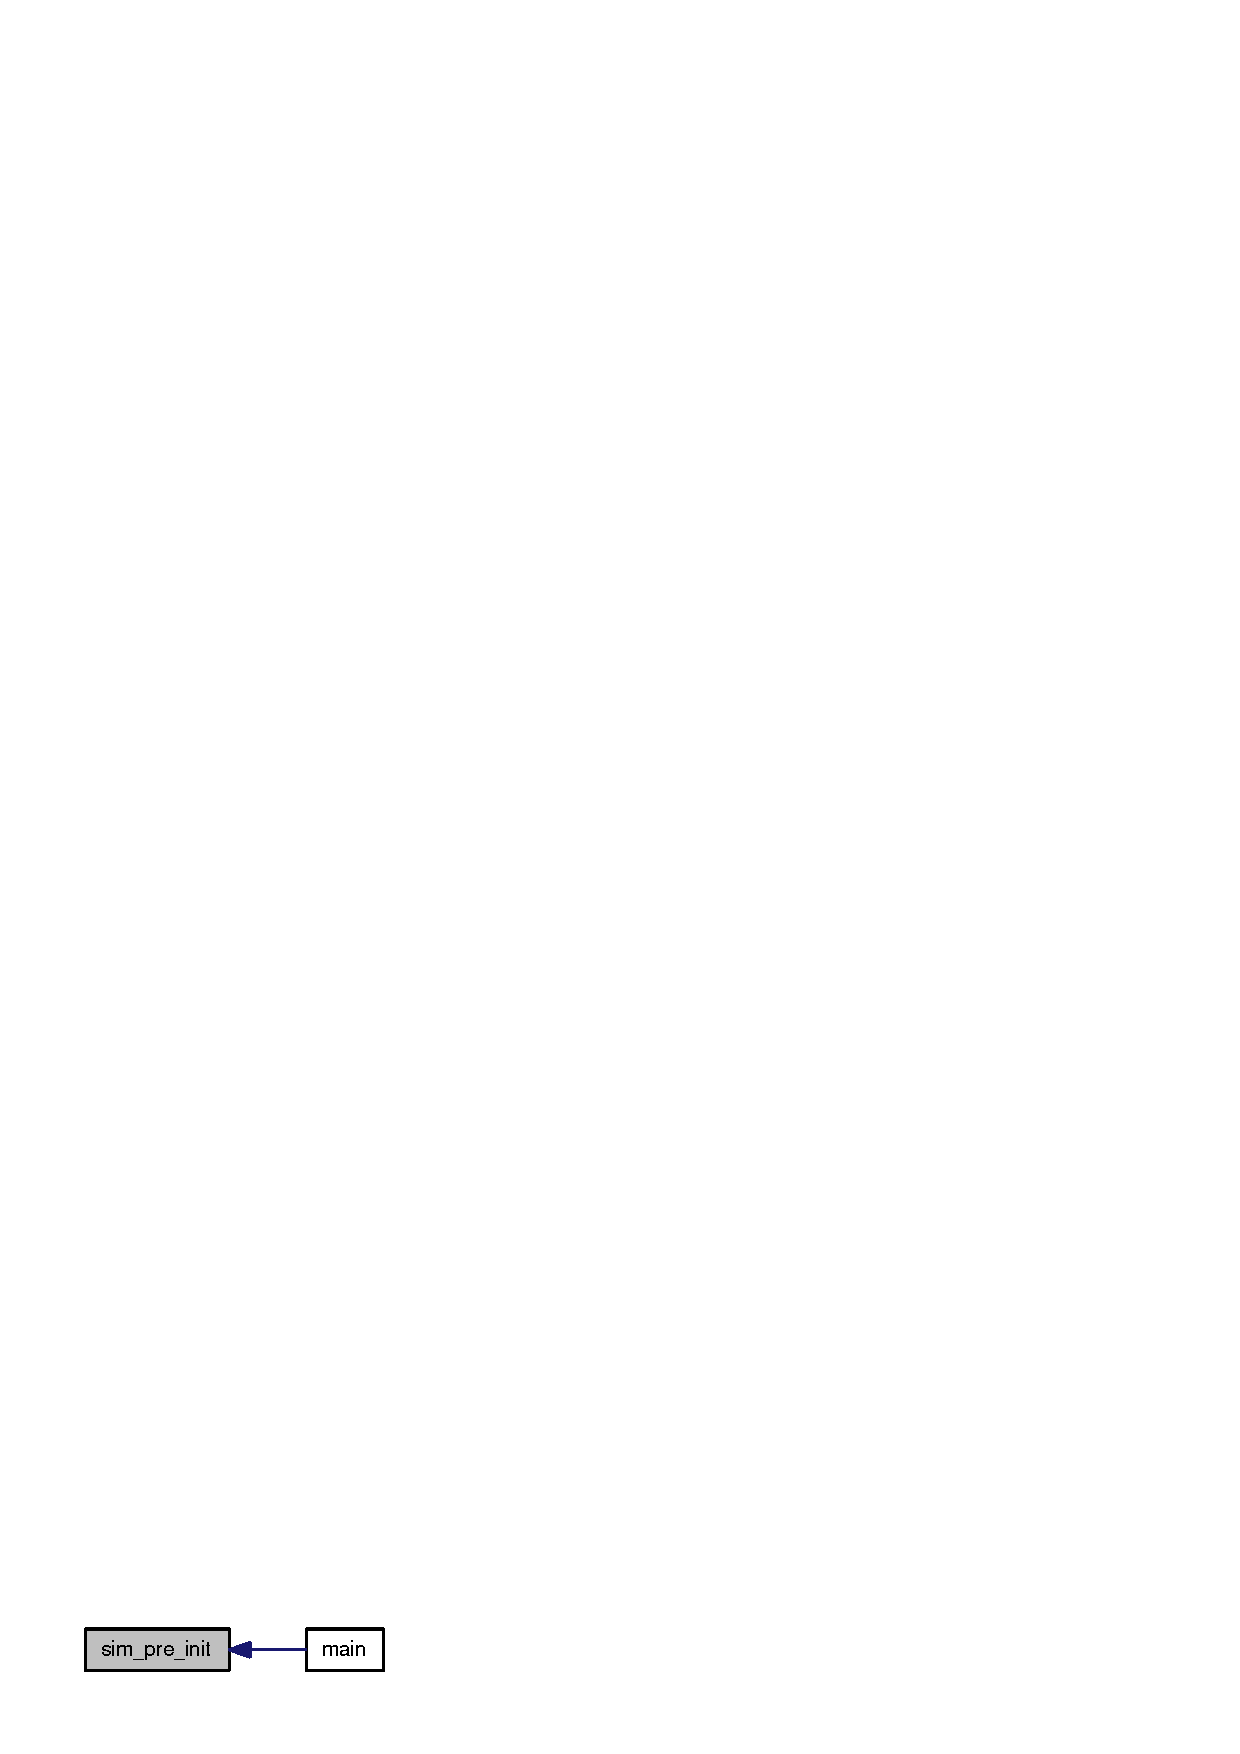
\includegraphics[width=94pt]{sim_8h_6f8bfcc0d1d039d6fb378af082656f6f_icgraph}
\end{center}
\end{figure}
\index{sim.h@{sim.h}!sim\_\-print\_\-stats@{sim\_\-print\_\-stats}}
\index{sim\_\-print\_\-stats@{sim\_\-print\_\-stats}!sim.h@{sim.h}}
\subsubsection[{sim\_\-print\_\-stats}]{\setlength{\rightskip}{0pt plus 5cm}void sim\_\-print\_\-stats (FILE $\ast$ {\em fd})}\label{sim_8h_ebded8bcfea50ac2770a680b87509424}




Definition at line 164 of file manifold\_\-fullsim.cc.

References Mesh::interfaces, Mesh::link\_\-a, Mesh::link\_\-b, links, MAX, max\_\-phy\_\-link\_\-bits, max\_\-sim\_\-time, no\_\-nodes, running, sim\_\-aux\_\-stats(), sim\_\-elapsed\_\-time, sim\_\-end\_\-time, and sim\_\-start\_\-time.

Referenced by exit\_\-now(), and main().

Here is the caller graph for this function:\nopagebreak
\begin{figure}[H]
\begin{center}
\leavevmode
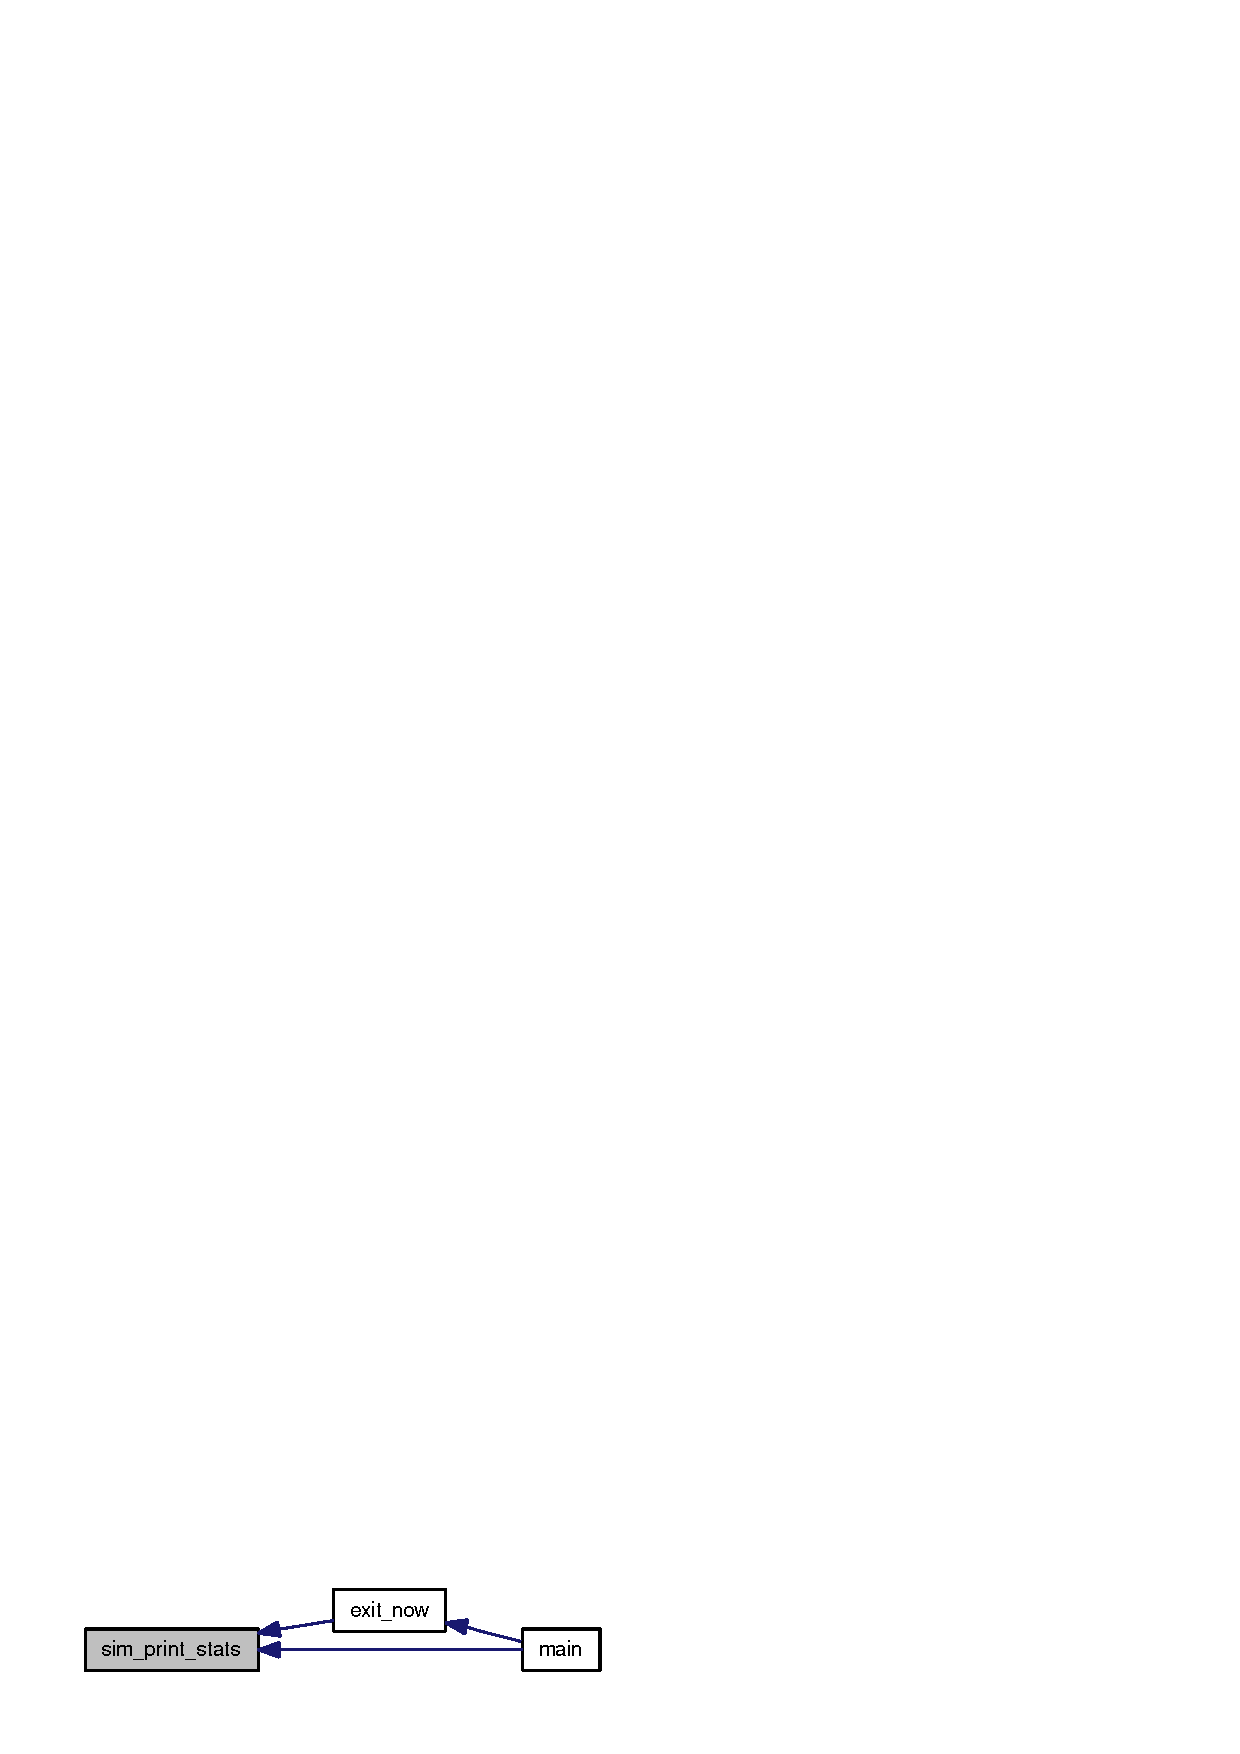
\includegraphics[width=146pt]{sim_8h_ebded8bcfea50ac2770a680b87509424_icgraph}
\end{center}
\end{figure}
\index{sim.h@{sim.h}!sim\_\-reg\_\-options@{sim\_\-reg\_\-options}}
\index{sim\_\-reg\_\-options@{sim\_\-reg\_\-options}!sim.h@{sim.h}}
\subsubsection[{sim\_\-reg\_\-options}]{\setlength{\rightskip}{0pt plus 5cm}void sim\_\-reg\_\-options (struct {\bf opt\_\-odb\_\-t} $\ast$ {\em odb})}\label{sim_8h_4452f31e857cb0adc1cd9ecc3be5f2ee}




Referenced by main().

Here is the caller graph for this function:\nopagebreak
\begin{figure}[H]
\begin{center}
\leavevmode
\includegraphics[width=103pt]{sim_8h_4452f31e857cb0adc1cd9ecc3be5f2ee_icgraph}
\end{center}
\end{figure}
\index{sim.h@{sim.h}!sim\_\-reg\_\-stats@{sim\_\-reg\_\-stats}}
\index{sim\_\-reg\_\-stats@{sim\_\-reg\_\-stats}!sim.h@{sim.h}}
\subsubsection[{sim\_\-reg\_\-stats}]{\setlength{\rightskip}{0pt plus 5cm}void sim\_\-reg\_\-stats (struct {\bf thread\_\-t} $\ast$$\ast$ {\em cores}, \/  struct {\bf stat\_\-sdb\_\-t} $\ast$ {\em sdb})}\label{sim_8h_e59ed09fba74951f34eea93edae2e721}




Referenced by main().

Here is the caller graph for this function:\nopagebreak
\begin{figure}[H]
\begin{center}
\leavevmode
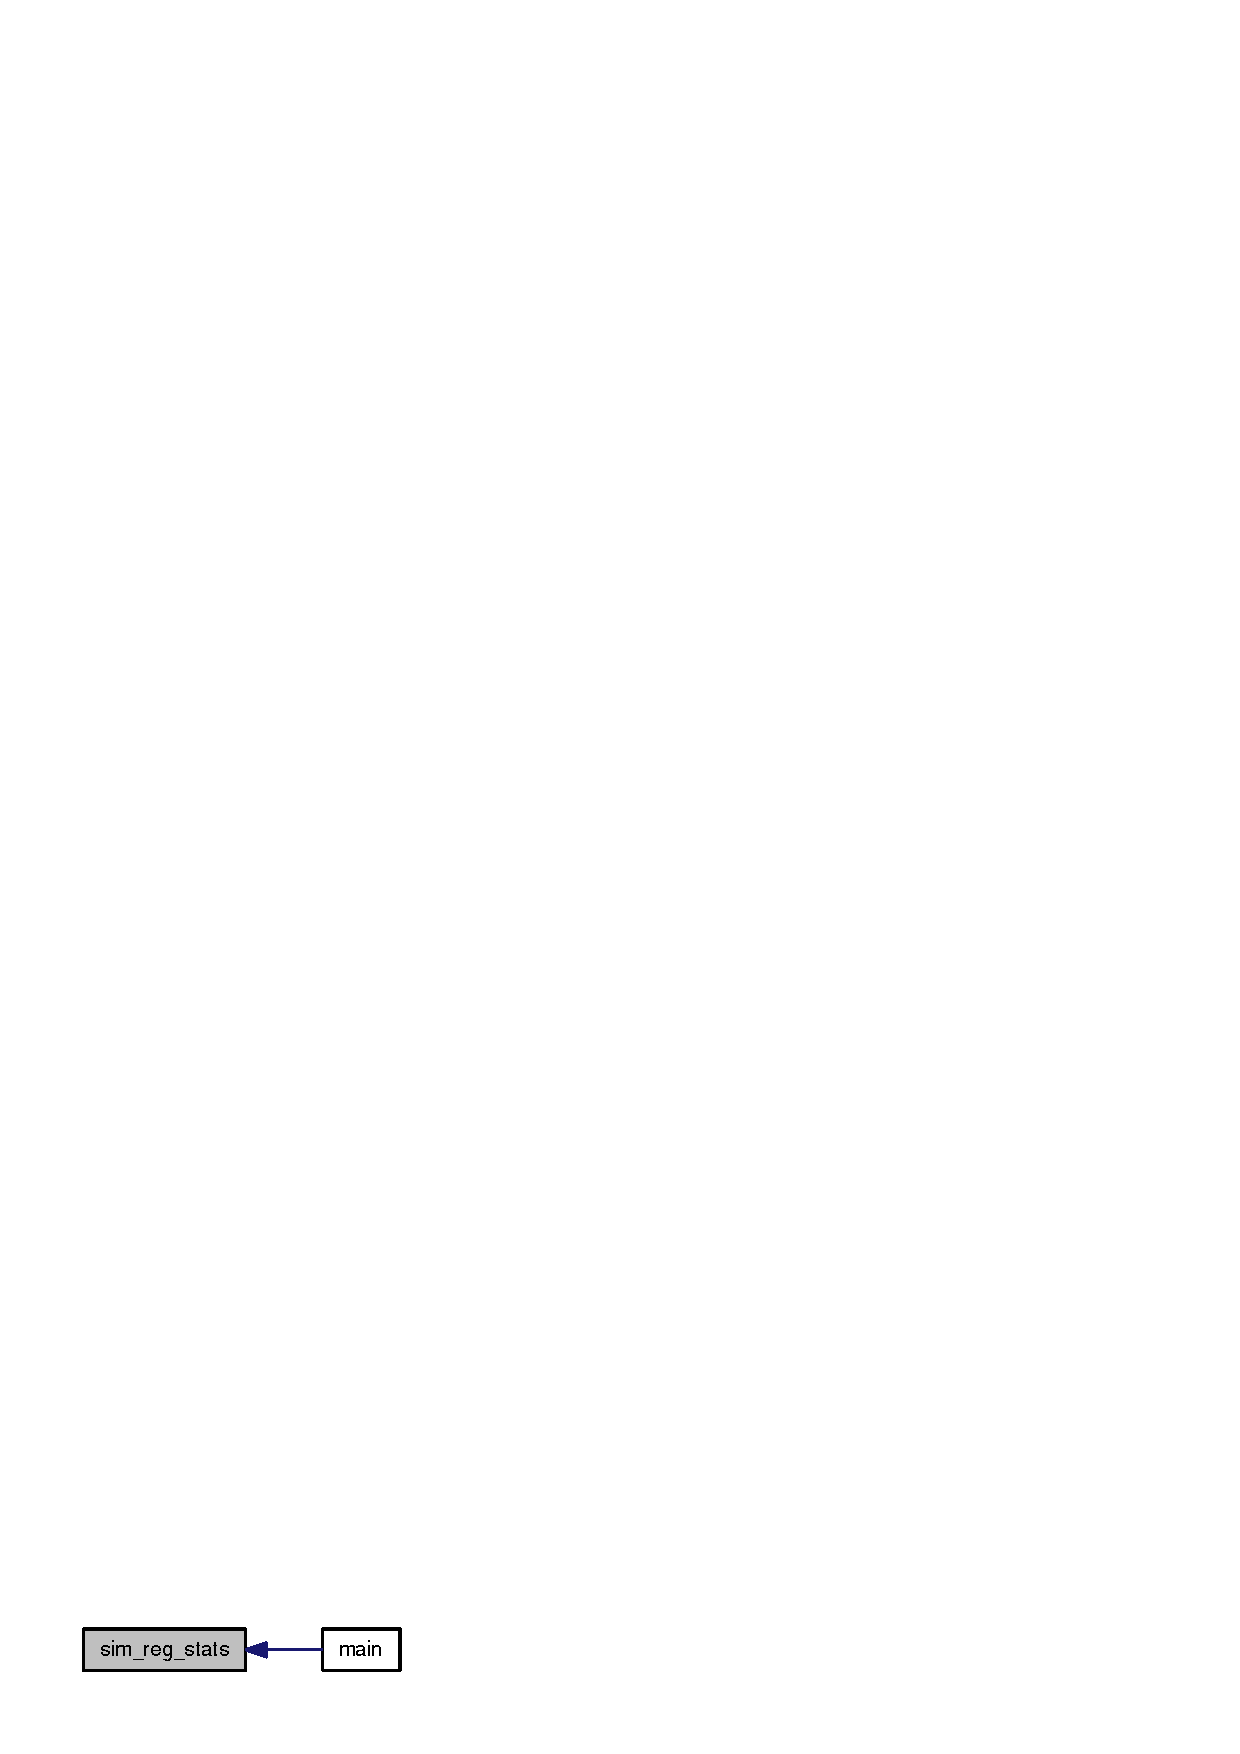
\includegraphics[width=98pt]{sim_8h_e59ed09fba74951f34eea93edae2e721_icgraph}
\end{center}
\end{figure}
\index{sim.h@{sim.h}!sim\_\-uninit@{sim\_\-uninit}}
\index{sim\_\-uninit@{sim\_\-uninit}!sim.h@{sim.h}}
\subsubsection[{sim\_\-uninit}]{\setlength{\rightskip}{0pt plus 5cm}void sim\_\-uninit (void)}\label{sim_8h_12f418d794abd0896d834c9582373b00}




Definition at line 437 of file sim-zesto.cpp.

\subsection{Variable Documentation}
\index{sim.h@{sim.h}!BANK\_\-BITS@{BANK\_\-BITS}}
\index{BANK\_\-BITS@{BANK\_\-BITS}!sim.h@{sim.h}}
\subsubsection[{BANK\_\-BITS}]{\setlength{\rightskip}{0pt plus 5cm}unsigned int {\bf BANK\_\-BITS}}\label{sim_8h_4dead09fbe9da04753765df2d1dc54dd}




Definition at line 38 of file config\_\-constants.h.\index{sim.h@{sim.h}!buffer\_\-size@{buffer\_\-size}}
\index{buffer\_\-size@{buffer\_\-size}!sim.h@{sim.h}}
\subsubsection[{buffer\_\-size}]{\setlength{\rightskip}{0pt plus 5cm}unsigned int {\bf buffer\_\-size}}\label{sim_8h_2a0484a5686f3c473e720462aba197bb}




Definition at line 48 of file config\_\-params.h.

Referenced by dump\_\-configuration(), iris\_\-init(), iris\_\-process\_\-options(), and main().\index{sim.h@{sim.h}!cores\_\-per\_\-node@{cores\_\-per\_\-node}}
\index{cores\_\-per\_\-node@{cores\_\-per\_\-node}!sim.h@{sim.h}}
\subsubsection[{cores\_\-per\_\-node}]{\setlength{\rightskip}{0pt plus 5cm}unsigned int {\bf cores\_\-per\_\-node}}\label{sim_8h_d1fe1c89980f30a3204e89fe23449677}




Definition at line 48 of file manifold\_\-fullsim.cc.

Referenced by iris\_\-process\_\-options(), main(), sim\_\-post\_\-init(), and uncore\_\-t::uncore\_\-t().\index{sim.h@{sim.h}!cpu\_\-speed@{cpu\_\-speed}}
\index{cpu\_\-speed@{cpu\_\-speed}!sim.h@{sim.h}}
\subsubsection[{cpu\_\-speed}]{\setlength{\rightskip}{0pt plus 5cm}double {\bf cpu\_\-speed}}\label{sim_8h_ebb0be7596a98356724d9653c17116c2}




Definition at line 176 of file sim-zesto.cpp.

Referenced by sim\_\-post\_\-init(), and uncore\_\-reg\_\-options().\index{sim.h@{sim.h}!credits@{credits}}
\index{credits@{credits}!sim.h@{sim.h}}
\subsubsection[{credits}]{\setlength{\rightskip}{0pt plus 5cm}unsigned int {\bf credits}}\label{sim_8h_75e66776a25c2fa845e1ba85ac6329ef}




Definition at line 48 of file config\_\-params.h.

Referenced by dump\_\-configuration(), iris\_\-init(), iris\_\-process\_\-options(), and main().\index{sim.h@{sim.h}!do\_\-two\_\-stage\_\-router@{do\_\-two\_\-stage\_\-router}}
\index{do\_\-two\_\-stage\_\-router@{do\_\-two\_\-stage\_\-router}!sim.h@{sim.h}}
\subsubsection[{do\_\-two\_\-stage\_\-router}]{\setlength{\rightskip}{0pt plus 5cm}unsigned int {\bf do\_\-two\_\-stage\_\-router}}\label{sim_8h_f584a3fbd576b0061c6c726603cea3e4}




Definition at line 32 of file config\_\-params.h.\index{sim.h@{sim.h}!grid\_\-size@{grid\_\-size}}
\index{grid\_\-size@{grid\_\-size}!sim.h@{sim.h}}
\subsubsection[{grid\_\-size}]{\setlength{\rightskip}{0pt plus 5cm}unsigned int {\bf grid\_\-size}}\label{sim_8h_850e232aff3d3acf04c7d39346f0bf4c}




Definition at line 44 of file config\_\-params.h.\index{sim.h@{sim.h}!help\_\-me@{help\_\-me}}
\index{help\_\-me@{help\_\-me}!sim.h@{sim.h}}
\subsubsection[{help\_\-me}]{\setlength{\rightskip}{0pt plus 5cm}bool {\bf help\_\-me}}\label{sim_8h_98b74f22826e26c7727ce84f6d3a621b}




Definition at line 108 of file manifold\_\-fullsim.cc.

Referenced by main().\index{sim.h@{sim.h}!init\_\-quit@{init\_\-quit}}
\index{init\_\-quit@{init\_\-quit}!sim.h@{sim.h}}
\subsubsection[{init\_\-quit}]{\setlength{\rightskip}{0pt plus 5cm}bool {\bf init\_\-quit}}\label{sim_8h_1d93ba7fce2ae0edcb3665632a12bd49}




Definition at line 114 of file manifold\_\-fullsim.cc.

Referenced by main().\index{sim.h@{sim.h}!max\_\-phy\_\-link\_\-bits@{max\_\-phy\_\-link\_\-bits}}
\index{max\_\-phy\_\-link\_\-bits@{max\_\-phy\_\-link\_\-bits}!sim.h@{sim.h}}
\subsubsection[{max\_\-phy\_\-link\_\-bits}]{\setlength{\rightskip}{0pt plus 5cm}unsigned int {\bf max\_\-phy\_\-link\_\-bits}}\label{sim_8h_81294da08255fbf06c1a30ee6d52059f}




Definition at line 33 of file config\_\-params.h.\index{sim.h@{sim.h}!max\_\-sim\_\-time@{max\_\-sim\_\-time}}
\index{max\_\-sim\_\-time@{max\_\-sim\_\-time}!sim.h@{sim.h}}
\subsubsection[{max\_\-sim\_\-time}]{\setlength{\rightskip}{0pt plus 5cm}unsigned long long int {\bf max\_\-sim\_\-time}}\label{sim_8h_35eb3b8621b39fb3b39217f5fb55bb31}




Definition at line 36 of file config\_\-params.h.\index{sim.h@{sim.h}!MC\_\-ADDR\_\-BITS@{MC\_\-ADDR\_\-BITS}}
\index{MC\_\-ADDR\_\-BITS@{MC\_\-ADDR\_\-BITS}!sim.h@{sim.h}}
\subsubsection[{MC\_\-ADDR\_\-BITS}]{\setlength{\rightskip}{0pt plus 5cm}unsigned int {\bf MC\_\-ADDR\_\-BITS}}\label{sim_8h_5797f7fc969d8a7c02df4ba708ed734f}




Definition at line 37 of file config\_\-constants.h.\index{sim.h@{sim.h}!nice\_\-priority@{nice\_\-priority}}
\index{nice\_\-priority@{nice\_\-priority}!sim.h@{sim.h}}
\subsubsection[{nice\_\-priority}]{\setlength{\rightskip}{0pt plus 5cm}int {\bf nice\_\-priority}}\label{sim_8h_1cb688b2b9eda644e545e25f039761e4}




Definition at line 117 of file manifold\_\-fullsim.cc.

Referenced by main().\index{sim.h@{sim.h}!no\_\-mcs@{no\_\-mcs}}
\index{no\_\-mcs@{no\_\-mcs}!sim.h@{sim.h}}
\subsubsection[{no\_\-mcs}]{\setlength{\rightskip}{0pt plus 5cm}unsigned int {\bf no\_\-mcs}}\label{sim_8h_544ce85a29feb73c485a704009deffd1}




Definition at line 31 of file config\_\-params.h.\index{sim.h@{sim.h}!no\_\-nodes@{no\_\-nodes}}
\index{no\_\-nodes@{no\_\-nodes}!sim.h@{sim.h}}
\subsubsection[{no\_\-nodes}]{\setlength{\rightskip}{0pt plus 5cm}unsigned int {\bf no\_\-nodes}}\label{sim_8h_e6ac8ea6f14ad67a94df03963a6613d1}




Definition at line 30 of file config\_\-params.h.\index{sim.h@{sim.h}!ports@{ports}}
\index{ports@{ports}!sim.h@{sim.h}}
\subsubsection[{ports}]{\setlength{\rightskip}{0pt plus 5cm}unsigned int {\bf ports}}\label{sim_8h_e9035ab8a30b22227c82949064511570}




Definition at line 48 of file config\_\-params.h.

Referenced by dump\_\-configuration(), iris\_\-init(), iris\_\-process\_\-options(), and main().\index{sim.h@{sim.h}!print\_\-setup@{print\_\-setup}}
\index{print\_\-setup@{print\_\-setup}!sim.h@{sim.h}}
\subsubsection[{print\_\-setup}]{\setlength{\rightskip}{0pt plus 5cm}unsigned int {\bf print\_\-setup}}\label{sim_8h_be380a7655f74438bdbac99614e71655}




Definition at line 43 of file config\_\-params.h.

Referenced by iris\_\-init(), iris\_\-process\_\-options(), and main().\index{sim.h@{sim.h}!rand\_\-seed@{rand\_\-seed}}
\index{rand\_\-seed@{rand\_\-seed}!sim.h@{sim.h}}
\subsubsection[{rand\_\-seed}]{\setlength{\rightskip}{0pt plus 5cm}int {\bf rand\_\-seed}}\label{sim_8h_b58df36fd429cab6ab2f2dedd531f7a9}




Definition at line 111 of file manifold\_\-fullsim.cc.

Referenced by main().\index{sim.h@{sim.h}!sim\_\-dump\_\-stats@{sim\_\-dump\_\-stats}}
\index{sim\_\-dump\_\-stats@{sim\_\-dump\_\-stats}!sim.h@{sim.h}}
\subsubsection[{sim\_\-dump\_\-stats}]{\setlength{\rightskip}{0pt plus 5cm}int {\bf sim\_\-dump\_\-stats}}\label{sim_8h_5f0267e6bed91a9151ebcc5e0a7557dc}




Definition at line 91 of file manifold\_\-fullsim.cc.

Referenced by signal\_\-sim\_\-stats().\index{sim.h@{sim.h}!sim\_\-eio\_\-fd@{sim\_\-eio\_\-fd}}
\index{sim\_\-eio\_\-fd@{sim\_\-eio\_\-fd}!sim.h@{sim.h}}
\subsubsection[{sim\_\-eio\_\-fd}]{\setlength{\rightskip}{0pt plus 5cm}FILE$\ast$ {\bf sim\_\-eio\_\-fd}[MAX\_\-CORES]}\label{sim_8h_10ca7f1cb78d9d34e56b67ac6c202480}


\index{sim.h@{sim.h}!sim\_\-eio\_\-fname@{sim\_\-eio\_\-fname}}
\index{sim\_\-eio\_\-fname@{sim\_\-eio\_\-fname}!sim.h@{sim.h}}
\subsubsection[{sim\_\-eio\_\-fname}]{\setlength{\rightskip}{0pt plus 5cm}char$\ast$ {\bf sim\_\-eio\_\-fname}[MAX\_\-CORES]}\label{sim_8h_ba89c3962ef5804b8fc49427a39269f7}


\index{sim.h@{sim.h}!sim\_\-elapsed\_\-time@{sim\_\-elapsed\_\-time}}
\index{sim\_\-elapsed\_\-time@{sim\_\-elapsed\_\-time}!sim.h@{sim.h}}
\subsubsection[{sim\_\-elapsed\_\-time}]{\setlength{\rightskip}{0pt plus 5cm}int {\bf sim\_\-elapsed\_\-time}}\label{sim_8h_84462569a8ea1951d2547b98eaa30f25}




Definition at line 78 of file manifold\_\-fullsim.cc.\index{sim.h@{sim.h}!sim\_\-end\_\-time@{sim\_\-end\_\-time}}
\index{sim\_\-end\_\-time@{sim\_\-end\_\-time}!sim.h@{sim.h}}
\subsubsection[{sim\_\-end\_\-time}]{\setlength{\rightskip}{0pt plus 5cm}time\_\-t {\bf sim\_\-end\_\-time}}\label{sim_8h_5db757faa4910d3f30bfddc7c81261e8}




Definition at line 77 of file manifold\_\-fullsim.cc.

Referenced by sim\_\-print\_\-stats().\index{sim.h@{sim.h}!sim\_\-exit\_\-buf@{sim\_\-exit\_\-buf}}
\index{sim\_\-exit\_\-buf@{sim\_\-exit\_\-buf}!sim.h@{sim.h}}
\subsubsection[{sim\_\-exit\_\-buf}]{\setlength{\rightskip}{0pt plus 5cm}jmp\_\-buf {\bf sim\_\-exit\_\-buf}}\label{sim_8h_84727c65b24d2e32fd3d4a7af53aa15a}




Definition at line 88 of file manifold\_\-fullsim.cc.

Referenced by main(), md\_\-fetch\_\-inst(), core\_\-commit\_\-STM\_\-t::step(), and core\_\-commit\_\-DPM\_\-t::step().\index{sim.h@{sim.h}!sim\_\-exit\_\-now@{sim\_\-exit\_\-now}}
\index{sim\_\-exit\_\-now@{sim\_\-exit\_\-now}!sim.h@{sim.h}}
\subsubsection[{sim\_\-exit\_\-now}]{\setlength{\rightskip}{0pt plus 5cm}int {\bf sim\_\-exit\_\-now}}\label{sim_8h_e6c582e7e1a51970f03ee0c8bb8776df}




Definition at line 85 of file manifold\_\-fullsim.cc.

Referenced by signal\_\-exit\_\-now().\index{sim.h@{sim.h}!sim\_\-odb@{sim\_\-odb}}
\index{sim\_\-odb@{sim\_\-odb}!sim.h@{sim.h}}
\subsubsection[{sim\_\-odb}]{\setlength{\rightskip}{0pt plus 5cm}struct {\bf opt\_\-odb\_\-t}$\ast$ {\bf sim\_\-odb}}\label{sim_8h_5520d419f4ed203a8f4496330bef06e3}




Definition at line 94 of file manifold\_\-fullsim.cc.\index{sim.h@{sim.h}!sim\_\-progfd@{sim\_\-progfd}}
\index{sim\_\-progfd@{sim\_\-progfd}!sim.h@{sim.h}}
\subsubsection[{sim\_\-progfd}]{\setlength{\rightskip}{0pt plus 5cm}FILE$\ast$ {\bf sim\_\-progfd}}\label{sim_8h_f93f90c77918d1b430318725f0f607a8}




Definition at line 102 of file manifold\_\-fullsim.cc.

Referenced by main().\index{sim.h@{sim.h}!sim\_\-progout@{sim\_\-progout}}
\index{sim\_\-progout@{sim\_\-progout}!sim.h@{sim.h}}
\subsubsection[{sim\_\-progout}]{\setlength{\rightskip}{0pt plus 5cm}char$\ast$ {\bf sim\_\-progout}}\label{sim_8h_21fe317600267fa77e054df4355779dc}




Definition at line 101 of file manifold\_\-fullsim.cc.

Referenced by main().\index{sim.h@{sim.h}!sim\_\-sdb@{sim\_\-sdb}}
\index{sim\_\-sdb@{sim\_\-sdb}!sim.h@{sim.h}}
\subsubsection[{sim\_\-sdb}]{\setlength{\rightskip}{0pt plus 5cm}struct {\bf stat\_\-sdb\_\-t}$\ast$ {\bf sim\_\-sdb}}\label{sim_8h_2f46df2af0ce568e5ae2ea2a78cb006b}




Definition at line 97 of file manifold\_\-fullsim.cc.\index{sim.h@{sim.h}!sim\_\-simout@{sim\_\-simout}}
\index{sim\_\-simout@{sim\_\-simout}!sim.h@{sim.h}}
\subsubsection[{sim\_\-simout}]{\setlength{\rightskip}{0pt plus 5cm}char$\ast$ {\bf sim\_\-simout}}\label{sim_8h_09cbb844712d19de24f7ec8a414d4266}




Definition at line 100 of file manifold\_\-fullsim.cc.

Referenced by main().\index{sim.h@{sim.h}!sim\_\-start\_\-time@{sim\_\-start\_\-time}}
\index{sim\_\-start\_\-time@{sim\_\-start\_\-time}!sim.h@{sim.h}}
\subsubsection[{sim\_\-start\_\-time}]{\setlength{\rightskip}{0pt plus 5cm}time\_\-t {\bf sim\_\-start\_\-time}}\label{sim_8h_e8d0794b6bec1dfbd28ca90a7a08d2b4}




Definition at line 76 of file manifold\_\-fullsim.cc.

Referenced by main(), sim\_\-main(), and sim\_\-print\_\-stats().\index{sim.h@{sim.h}!sim\_\-swap\_\-bytes@{sim\_\-swap\_\-bytes}}
\index{sim\_\-swap\_\-bytes@{sim\_\-swap\_\-bytes}!sim.h@{sim.h}}
\subsubsection[{sim\_\-swap\_\-bytes}]{\setlength{\rightskip}{0pt plus 5cm}int {\bf sim\_\-swap\_\-bytes}}\label{sim_8h_feede3aab9267fb42b819ad7bc47247a}




Definition at line 81 of file manifold\_\-fullsim.cc.\index{sim.h@{sim.h}!sim\_\-swap\_\-words@{sim\_\-swap\_\-words}}
\index{sim\_\-swap\_\-words@{sim\_\-swap\_\-words}!sim.h@{sim.h}}
\subsubsection[{sim\_\-swap\_\-words}]{\setlength{\rightskip}{0pt plus 5cm}int {\bf sim\_\-swap\_\-words}}\label{sim_8h_a1267d1f1ee712bf4d37a9f7c4d2e913}




Definition at line 82 of file manifold\_\-fullsim.cc.\index{sim.h@{sim.h}!THREAD\_\-BITS\_\-POSITION@{THREAD\_\-BITS\_\-POSITION}}
\index{THREAD\_\-BITS\_\-POSITION@{THREAD\_\-BITS\_\-POSITION}!sim.h@{sim.h}}
\subsubsection[{THREAD\_\-BITS\_\-POSITION}]{\setlength{\rightskip}{0pt plus 5cm}unsigned int {\bf THREAD\_\-BITS\_\-POSITION}}\label{sim_8h_581f0c063e972c5f202149f2e3ce7452}




Definition at line 36 of file config\_\-constants.h.\index{sim.h@{sim.h}!vcs@{vcs}}
\index{vcs@{vcs}!sim.h@{sim.h}}
\subsubsection[{vcs}]{\setlength{\rightskip}{0pt plus 5cm}unsigned int {\bf vcs}}\label{sim_8h_7ef93ae807d4d29652202027711634cf}




Definition at line 48 of file config\_\-params.h.

Referenced by dump\_\-configuration(), uncore\_\-t::enqueuable(), iris\_\-init(), iris\_\-process\_\-options(), main(), and sim\_\-post\_\-init().